\documentclass[letterpaper]{deedy-resume} % Use US Letter paper, change to a4paper for A4 

\begin{document}

%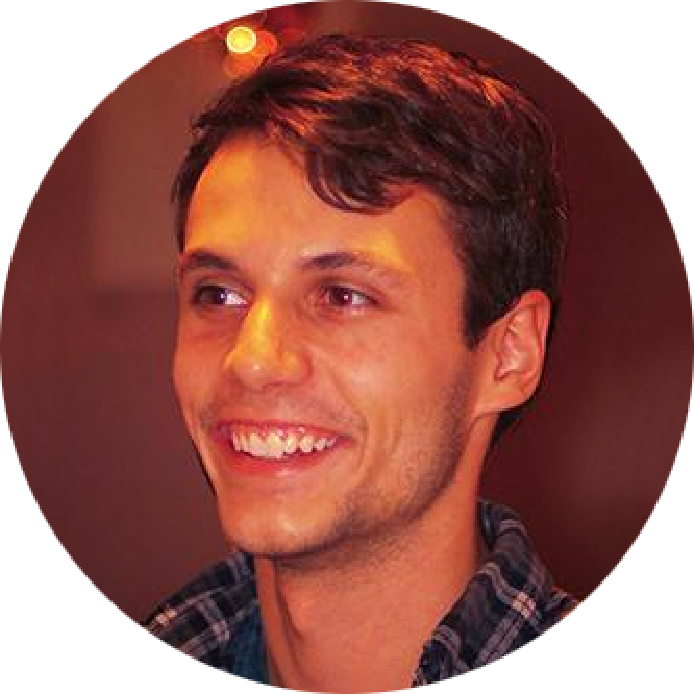
\includegraphics[scale=0.25]{linkedin}

\namesection{}{Ethan Russell}{ % Your name
\href{mailto:ethan@ethan-russell.com}{ethan@ethan-russell.com} | \href{http://ethan-russell.com}{ethan-russell.com} | 503.757.8103 % Your contact information
}
\begin{minipage}[t]{0.33\textwidth} % The left column takes up 33% of the text width of the page

%------------------------------------------------
% Education
%------------------------------------------------
\section{}
\begin{center}
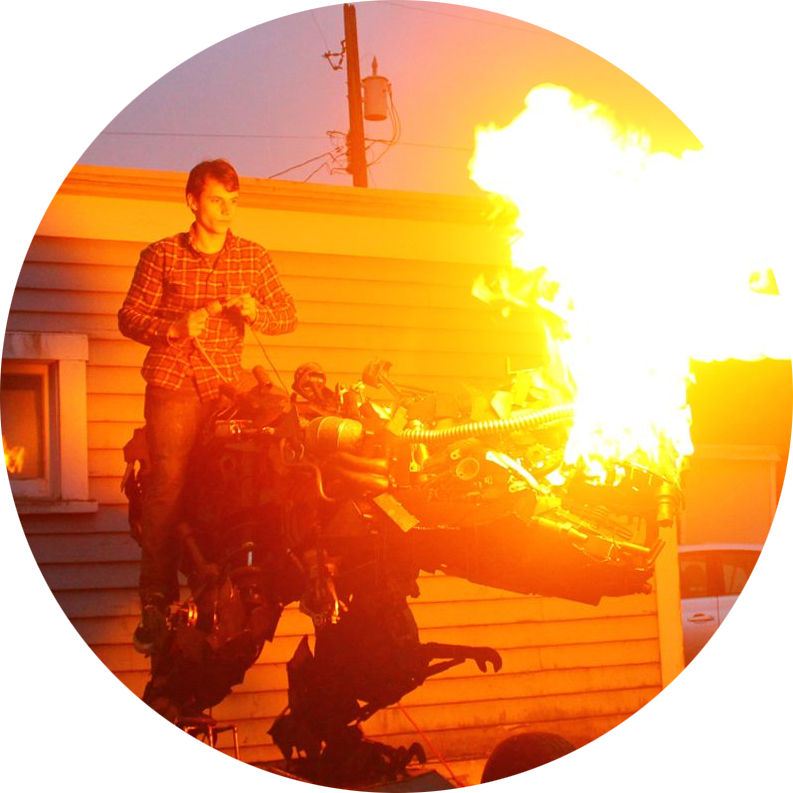
\includegraphics[scale=0.2]{profile.png}
\end{center}

\section{Summary}
\descript{Creative, self-motivated, and passionate engineer driven to solve problems and create novel new ideas.}

\sectionspace % Some whitespace after the section

\section{Education} 

\descript{University of Puget Sound}

\descript{B.S. in Computer Science}
Graduated May 2017 | Tacoma, WA

\sectionspace % Some whitespace after the section

\section{Skills}
\sectionspace % Some whitespace after the section

\begin{tightitemize}

\item
Software Development \newline(Embedded: C, C++, \newline Desktop: Qt, .Net)

\item
STM32 Ecosystem: Cube, TouchGFX

\item
PCB design and layout (Altium Designer)

\item
Power Electronics Design and Controls

\item
Electromechanical System Design

\end{tightitemize}

\sectionspace % Some whitespace after the section

\section{About} 
\sectionspace % Some whitespace after the section
My work specializes in embedded systems, but I enjoy the breadth of skills involved with creating something from scratch: CNC machining, computer graphics, metal fabrication.  See my website for a portfolio of personal projects.
\end{minipage} % The end of the left column
\hfill
%
%----------------------------------------------------------------------------------------
%	RIGHT COLUMN
%----------------------------------------------------------------------------------------
%
\begin{minipage}[t]{0.66\textwidth} % The right column takes up 66% of the text width of the page

%------------------------------------------------
% Experience
%------------------------------------------------

\sectionspace % Some whitespace after the section

\section{Work Experience}

\runsubsection{Chapman Leonard}
\descript{| Firmware/EE/Systems Consultant}
\location{Dec. 2023 - Present | North Hollywood, CA}
\vspace{\topsep} % Hacky fix for awkward extra vertical space
\begin{tightitemize}
\item 
Hired as a consultant to spearhead upgrading traditional video production studio equipment to software control.

\item
Responsible for systems design, power-electronics design, high reliability real-time firmware, UI firmware, and systems integration for version 2 of an 8000 pound hydraulic/electric studio crane base to run IMU-based hydraulic post-stabilization, servo drive for repeated movements, and wireless console for user control.

\item 
Designed circuit boards, created firmware/bootloader suite, and produced a small production run of a camera-head "Mini-Console" with touch screen interface created using ST TouchGFX.  Created a series of user-interface devices and associated electronics and firmware to interface with the Mini-Console.

\item Coordinated a small team of mechanical engineers for electro-mechanical upgrades to existing bases.

\end{tightitemize}

\runsubsection{Freefly Systems}
\descript{| Robotics Engineer}
\location{July 2017 - June 2022 | Woodinville, WA}
\begin{tightitemize}
\item 
Involved in system design, electrical design and software development of medium-volume (prosumer) products, including:

- \textit{Industrial Gimbal Payloads}: Owned the system design, electrical and software design and development, and production processes for a new gimbal framework, and PX4 aircraft integration for Astro.

- \textit{Astro}, a drone aimed at industrial applications: Electrical design and PCB layout, and application/bootloader firmware development/validation of a high reliability field-oriented brushless motor drive. 

- \textit{MoVI Ecosystem}: Owned firmware development of Freefly's cinema-grade gimbals and controllers including a major software revamp that introduced many new features for existing customers.  For high-volume products, developed factory bringup fixtures and systems.

- \textit{Alta X}:  Motor telemetry module: in rapid response to a crash and recall, reverse-engineered a protocol for proprietary off-the-shelf motor drives and developed an electrical and software package for communicating with the aircraft.

\end{tightitemize}

\runsubsection{University of Puget Sound}
\descript{| Science Support Engineer}
\location{Sep. 2013 - May 2017 | Tacoma, WA}
\begin{tightitemize}
\item Supported the sciences at UPS by designing and maintaining research equipment
\item Projects include:

- \textit{String winder:} designed, fabricated, and programmed a computer controlled guitar string lathe for a research project, and the supporting equipment and software for analysis.  Co-authored paper with findings.

- \textit{Nitrogen Generator:} designed, fabricated, and programmed a computer controlled pressure-swing-absorption system for replacing nitrogen dewars in the UPS Chemistry department

- \textit{CNC Plasma Cutter:} built a CNC plasma cutter for use in the machine shop
\end{tightitemize}



\runsubsection{Digiwest, LLC}
\descript{| Engineer/Technician}
\location{Summer 2014 | Portland, OR}
\begin{tightitemize}
\item Involved with assembly, development, testing, and packaging of the Digiwest BlueMAC traffic data collector hardware

\item Designed and prototyped a version of the BlueMAC product for use in NEMA TS2 cabinets
\end{tightitemize}

\runsubsection{Misc.}
\location{Before 2013}
\begin{tightitemize}
\item Routeware - Special Product Engineering Consultant
\item Mentor Graphics - Software Development Intern
\item FIRST Robotics Technical Mentor

\end{tightitemize}

\end{minipage} % The end of the right column

%----------------------------------------------------------------------------------------
%	SECOND PAGE (EXAMPLE)
%----------------------------------------------------------------------------------------

%\newpage % Start a new page

%\begin{minipage}[t]{0.33\textwidth} % The left column takes up 33% of the text width of the page

%\section{Example Section}

%\end{minipage} % The end of the left column
%\hfill
%\begin{minipage}[t]{0.66\textwidth} % The right column takes up 66% of the text width of the page

%\section{Example Section 2}

%\end{minipage} % The end of the right column

%----------------------------------------------------------------------------------------

\end{document}